\section{Sample indexed spatial orthogonal frequency division multiplexing}
\label{sec:sisofdm}

\graphicspath{{_MIMOSpace/figures_sisofdm/}}

%Recently, the increase in use of portable computing devices has created an intense demand for wireless data access. Spectral allocations and regulations limit our ability to increase the capacity of existing channels within the radio frequency (RF) spectrum. Advances made in the solid-state lighting industry are driving significant deployments of energy-efficient light emitting diode (LED) based luminaries. This has created an opportunity to use such luminaries to establish high capacity indoor visible light communication (VLC) links and reduce the bottleneck on existing RF wireless channels. Under this model, luminaries simultaneously support illumination and wireless data transmission \cite{elg11a}. OSM and O-OFDM are two techniques that have been proposed to implement such a dual-use VLC channel.

%OSM is a multiple-transmitter technique in which information is encoded over (a) index of luminiares that are spatially separated and (b) modulation scheme overlayed on indexed luminaire \cite{mes10a}. Within a symbol period, only one luminaire emits a radiant flux while all other luminaires are idle. This minimizes the inter-channel interference (ICI) thus simplifying the detection process and the overall system complexity as compared to spatial multiplexing (SMP). In OSM, the bit--stream to be transmitted is divided into contiguous sections of $k=$ log$^{ }_{2}(N_{\text{tx}})$ spatial bit--stream and $m=$ log$^{ }_{2}(M)$ modulation bit--stream where $N_{\text{tx}}$ is the number of luminaires and $M$ is the modulation order. The $k$ bits select the luminaire to be activated while the $m$ bits select the M-ary modulation symbol to be transmitted. Thus, OSM system provides $$ log$^{ }_{2}(MN_{\text{tx}})$ bits per symbol. In \cite{fat11a}, an OSM system with pulse amplitude modulation (PAM) as the overlayed modulation scheme is proposed. Reference \cite{pop12a} proposes a scheme that combines OSM with pulse position modulation (PPM) to benefit from the energy efficiency of PPM as compared to PAM. Reference \cite{but14a} shows imaging receiver can provide significant SNR gains for OSM and SMP as compared to non--imaging receiver.

\subsection{SIS-OFDM system outline}
\label{subsec:sisofdmSystem}

An approach to combine OSM and traditional OFDM is proposed in reference \cite{gan06a}. This approach is adapted for IM/DD communications in reference \cite{zha12a}. 
\afterpage{%
	\clearpage
	\begin{landscape}% Landscape page
		\begin{figure}[!t]
			\centering
			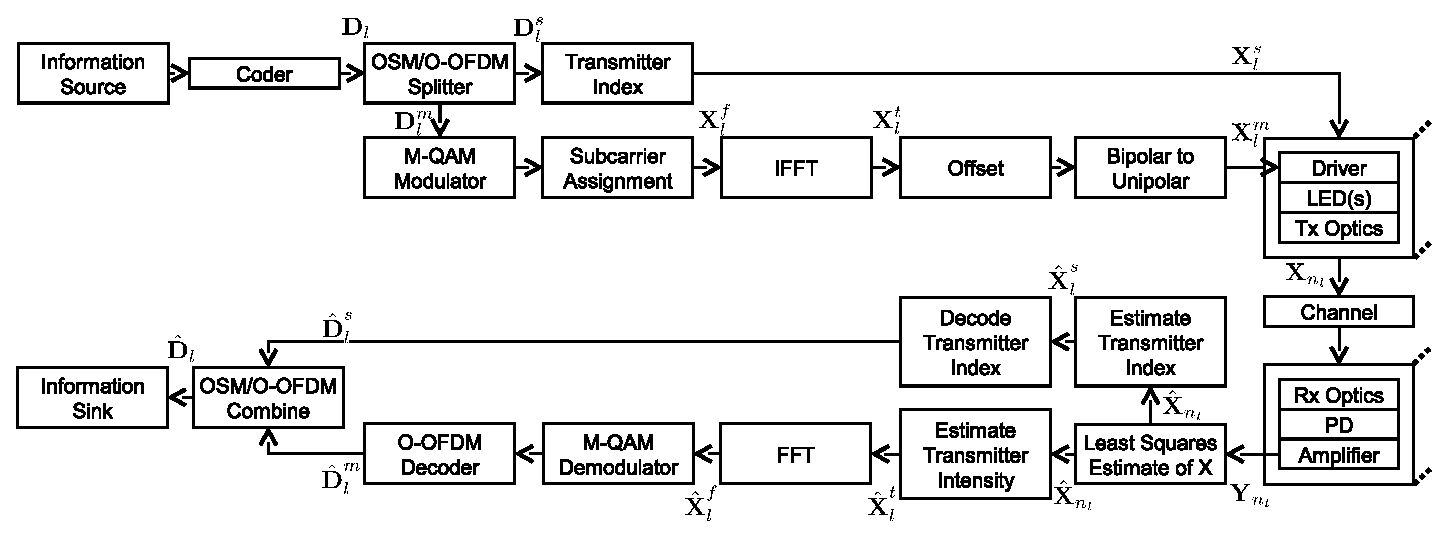
\includegraphics[trim={0.0in 0.0in 0.0in 0.0in}, clip=false, width=1.3\textwidth]{figBlockDiagram2.eps}
			\caption{Block diagram of system implementing SIS-OFDM}
			\label{figBlockDiagram}
		\end{figure}
	\end{landscape}
	\clearpage% Flush page
}
Here, an encoded information stream is divided into O-OFDM and OSM streams. Data from O-OFDM stream is assigned to different subcarriers to form the frequency domain O-OFDM symbol. OSM is then implemented in the frequency domain where each data--subcarrier is assigned to a transmitter determined by the encoded OSM stream. An IFFT operation is implemented at each transmitter to multiplex the data before transmission. Spectral efficiency of this scheme is then proportional to the number of data--subcarriers. In comparison, the spectral efficiency of SIS-OFDM is proportional to the number of total subcarriers which is equal to at least double the number of data--subcarriers. Additionally, the SIS-OFDM system requires a single IFFT operation, independent of the number of transmitters and thus maintains a computational complexity equal to that of SISO OFDM transmission. SIS-OFDM using an imaging receiver achieves much better power efficiency as compared to equivalent system using non--imaging receiver.

Implementation of SISO O-OFDM system is outlined in subsection \ref{subsec:sisoModulationOOFDM}. The number of data-subcarriers, $N_{\text{sc}}^{\text{d}}$, equals ($N_{\text{sc}}/4$) for ACO-OFDM and ($N_{\text{sc}}/2-1$) for DCO-OFDM where $N_{\text{sc}}$ is the total number of subcarriers. The number of transmitted bits per O-OFDM symbol is given by $R^{\text{m}}=N_{\text{sc}}^{\text{d}}\times $ log$^{ }_{2}(M)$. \figurename{\ref{figBlockDiagram}} illustrates the block diagram of a system implementing SIS-OFDM. The source generates the information to transmit. The coder encodes the information into a binary bit--stream $\vm{D}$ which is divided into consecutive segments of $R^{\text{ms}}=R^{\text{m}}+R^{\text{s}}$ bits where $R^{\text{s}}=N_{\text{sc}}\times k=N_{\text{sc}}\times $ log$^{ }_{2}(N_{\text{tx}})$ is the number of spatial bits. Let the $l^{th}$ such segment be denoted by $\vm{D}_l$. The first $R^{\text{m}}$ bits of $\vm{D}_l$ are collected in a vector $\vm{D}_l^{\text{m}}$ and are mapped to an $M$-QAM modulator. The generated QAM symbols are then assigned to subcarriers (based on the O-OFDM signal format, \textit{i.e.} DCO-OFDM or ACO-OFDM) to generate a frequency domain O-OFDM symbol $\vm{X}_l^{\text{f}}$ of length $N_{\text{sc}}$. An IFFT operation is applied on $\vm{X}_l^{\text{f}}$ to produce a real-valued bipolar time domain O-OFDM symbol $\vm{X}_l^{\text{t}}$ of the same length $N_{\text{sc}}$. The latter $R^{\text{s}}$ bits of $\vm{D}_l$ are collected in a vector $\vm{D}_{l}^{\text{s}}$ and are mapped to $N_{\text{sc}}$ length transmitter index vector denoted by $\vm{X}_l^{\text{s}}$. Let $\vm{X}_l^{\text{m}}$ denote the real unipolar baseband signal after biasing and/or clipping, and $0\leq n_l\leq (N_{\text{sc}}-1)$ indicate the relative time index for the next SIS-OFDM symbol to be transmitted. At each time instance, an O-OFDM signal value from $\vm{X}_l^{\text{m}}$ is transmitted from a luminaire indexed by $\vm{X}_l^{\text{s}}$. Let $\vm{X}_{n_l}$ be this $N_{\text{tx}}$ length transmission vector at time instant $n_l$. Thus the $j^{th}$ element of this vector is then given by
\begin{equation}
	\label{eqX}
	\vm{X}_{n_l}(j) = \twopartdef{\vm{X}_l^{\text{m}}(n_l)}{j=\vm{X}_l^{\text{s}}(n_l)}{0}{\text{else}}
\end{equation}

The SIS-OFDM symbol and transmit vector generation is explained using the following example which considers ACO-OFDM with $N_{\text{sc}}=8$, 4-QAM subcarrier modulation and $N_{\text{tx}}=2$. Here, $R^{\text{m}}=4$ and $R^{\text{s}}=8$, \textit{i.e} $R^{\text{ms}}=4+8=12$ bits per SIS-OFDM symbol. The assumed bits forming one SIS-OFDM symbol $\vm{D}_l$ are shown in Table \ref{tabExBits}. Table \ref{tabExample} then illustrates the data to subcarrier and transmitter index assignments. In this example, the transmitters would jointly transmit vector $\vm{X}_{n_l}=[0$ $\sqrt{2}]^{\text{T}}$ at relative time index $n_l=2$.
\begin{table}[!t]
	\centering
		\begin{tabular}{|c|l|}
			\hline
			{\bf{Stream}}&\multicolumn{1}{|c|}{\bf{Bits}}\\
			\hline
			$\vm{D}_l$ & $\left[\text{ 1 1 0 0 0 1 1 0 0 0 1 1 }\right]^{\text{t}} $\\
			\hline
			$\vm{D}_l^{\text{m}}$ & $\left[\text{ 1 1 0 0 }\right]^{\text{t}} $\\
			\hline
			$\vm{D}_l^{\text{s}}$ & $\left[\text{ 0 1 1 0 0 0 1 1 }\right]^{\text{t}} $\\
			\hline
		\end{tabular}
	\caption{Example SIS-OFDM data streams using ACO-OFDM}
	\label{tabExBits}
\end{table}

\begin{table}[!t]
	\centering
      \begin{tabular}{|c|c|c|c|c|c|c|}
			\hline
			{ $n_l$ }&{\bf{OFDM bits}}&$\vm{X}_l^{\text{f}}$&$\vm{X}^{\text{t}}_l$&$\vm{X}^{\text{m}}_l$&{\bf{SM bits}}&$\vm{X}^{\text{s}}_l$\\
			\hline
			0 & - & 0 & 0 & 0 &0 & 1\\
			\hline
			1 & 1 1 & $-1-j$ & $-1$ & 0 &1 & 2\\
			\hline
			2 & - & 0 & $\sqrt{2}$ & $\sqrt{2}$ &1 & 2\\
			\hline
			3 & 0 0 & $1+j$ & $1$ & $1$ & 0& 1\\
			\hline
			4 &-& 0 & 0 & 0 &0 & 1\\
			\hline
			5 &-& $1-j$ & $1$ & $1$ &0 & 1\\
			\hline
			6 &-& 0 & $-\sqrt{2}$ & 0 & 1& 2\\
			\hline
			7 &-& $-1+j$ & $-1$ & 0 &1 & 2\\
			\hline
		\end{tabular}
	\caption{Example subcarrier and luminaire assignment}
	\label{tabExample}
\end{table}

The indoor optical MIMO channel is modeled as,
\begin{equation}
	\label{eqChannel}
	\vm{Y}_{n_l} = \vm{H}\vm{X}_{n_l} + \vm{W}_{n_l}
\end{equation}
where $\vm{X}_{n_l}$ is the instantaneous transmit vector. $\vm{H}$ is the channel matrix and can be computed as in \cite{but13a}. $\vm{Y}_{n_l}$ is the received signal vector and $\vm{W}_{n_l}$ is zero-mean AWGN vector.

The receiver can be configured such that $\vm{H}$ is of rank $N_{\text{tx}}$. In that case, $(\vm{H}^{*}\vm{H})^{-1}$ exists. The least squares estimate of transmitted vector $\vm{X}_{n_l}$ can be computed as
\begin{equation}
	\label{eqXls}
	\hat{\vm{X}}_{n_l} = (\vm{H}^{*}\vm{H})^{-1}\vm{H}^{*}\vm{Y}_{n_l}
\end{equation}

In SIS-OFDM, only one luminaire emits radiant flux at a given time instance. Thus the maximum element of $\hat{\vm{X}}_{n_l}$ is estimated as the transmitted signal flux $\hat{x}^{\text{m}}_{n_l}$.
\begin{equation}
	\label{eqxhsym}
	\hat{x}^{\text{m}}_{n_l} = \max_{\forall j}\left(x_{j}\right); x_{j}\in\hat{\vm{X}}_{n_l}
\end{equation}

The index of $\hat{x}^{\text{m}}_{n_l}$ within $\hat{\vm{X}}_{n_l}$ provides an estimate of the active luminaire. Thus the instantaneous luminaire index $\hat{x}^{\text{s}}_{n_l}$ is estimated as
\begin{equation}
	\label{eqxhtx}
	\hat{x}^{\text{s}}_{n_l} = \idxmax_{\forall j}\left(x_{j}\right); x_{j}\in\hat{\vm{X}}_{n_l}
\end{equation}

A SIS-OFDM symbol is transmitted over $N_{\text{sc}}$ time slots. $\hat{x}^{\text{m}}_{n_l}$ and $\hat{x}^{\text{s}}_{n_l}$ are estimated for each time slot $n_l$ and collected in vectors $\hat{\vm{X}}^{\text{m}}_l$ and $\hat{\vm{X}}^{\text{s}}_l$ respectively. $\hat{\vm{X}}^{\text{m}}_l$ is subject to signal processing to recover the transmitted O-OFDM signal in $\hat{\vm{X}}^{\text{t}}_l$. An FFT process then demultiplexes the data and estimates the transmitted O-OFDM symbol in $\hat{\vm{X}}^{\text{f}}_l$. Maximum likelihood (ML) estimation is performed on the received symbols over the $N_{\text{sc}}^{\text{d}}$ data-subcarriers to estimate the bits transmitted and collected in $\hat{\vm{D}}^{\text{m}}_l$. The transmitter indexes estimated in $\hat{\vm{X}}^{\text{s}}_l$ are subject to decimal to $k$-length binary conversion to decode the spatial bits as $\hat{\vm{D}}^{\text{s}}_l$. The estimated OSM and O-OFDM bits are then combined to estimate the transmitted $l_{th}$ bit--stream as $\hat{\vm{D}}_l$.

The SIS-OFDM scheme explained above can provide up to $R^{\text{s}}$ additional bits per symbol over equivalent SISO O-OFDM transmission. The system explored in \cite{zha12a} can transmit $(N_{\text{sc}}^{\text{d}}\times k)$ spatial-bits per symbol as compared to $(N_{\text{sc}}\times k)$ spatial-bits per symbol in SIS-OFDM. Thus using SIS-OFDM provides additional spectral efficiency gain of ($3\times N_{\text{sc}}\times k/4$) bits per symbol while using ACO-OFDM and $((N_{\text{sc}}/2 -1)\times k)$ bits per symbol while using DCO-OFDM.

\subsection{SIS-OFDM system performance}
\label{subsec:sisofdmAnalysis}

Two comparable $4\times 4$ MIMO systems implementing SIS-OFDM with ACO-OFDM and DCO-OFDM are considered to evaluate the system performance using imaging and non--imaging receiver. The $N_{\text{tx}}=4$ lambertian transmitters of order 1 are assumed located on the ceiling of a room, facing vertically down, and at 0.5 m pitch. The transmitters are assumed to have a linear E/O conversion and transmit the upper peak signals without clipping. A 4-pixel imaging receiver with 1 mm pixel side length is assumed to have optics with 5 mm focal length, aperture of 1 mm$^2$ area and arranged in a $2\times 2$ grid. A 4-element non--imaging receiver is modeled to have 4 photodiodes of side length 1 mm, pitch of 1 mm, and a concentrator with 1.5 refractive index arranged in a $2\times 2$ grid. The receivers are assumed located in the center, facing upwards, and at a distance of 2 m from the transmitter plane. The transmitter side length is assumed small enough that its image lies entirely inside the corresponding pixel of the imaging receiver. Additionally, these MIMO systems are compared against an equivalent SISO system that receives the same amount of average optical flux as in the MIMO systems. 

In an indoor VLC environment, the propagation delay of light rays from luminaires to receiver is of the order of a few nano-seconds where as the modulation bandwidth is of the order of few tens of mega-Hertz. Additionally, the multipath reflected signals undergo path-loss of the order of 100dB as compared to LOS signals. Thus only LOS signals are considered. In such scenario, $\vm{H}$ with the imaging receiver is given by Eq. \eqref{eqHimr}, with non--imaging receiver is given by Eq. \eqref{eqHnimr} and for the SISO system is $0.8979\times 10^{-7}$. Note, in SIS-OFDM, since only 1 luminaire is active at a given time, the average transmitted flux per luminaire is assumed same as in the SISO system. Since all systems must receive the same amount of flux at same illumination levels, the point-to-point channel gains in each case are similar.
\begin{subequations}
\small
\begin{align}
	\vm{H} = 10^{-7}\times\left[
	                      \begin{array}{cccc}
												0&0&0&0.8979\\
												0&0&0.8979&0\\
												0&0.8979&0&0\\
												0.8979&0&0&0
												\end{array}
												\right]\label{eqHimr}\\
	\vm{H} = 10^{-7}\times\left[
	                      \begin{array}{cccc}
												0.8981&0.8979&0.8979&0.8977\\
												0.8979&0.8981&0.8977&0.8979\\
												0.8979&0.8977&0.8981&0.8979\\
												0.8977&0.8979&0.8979&0.8981
												\end{array}
												\right]\label{eqHnimr}
\end{align}
\label{eqH}
\end{subequations}
As mentioned before, for indoor VLC, transmitters must perform dual function of providing wireless data communication while maintaining appropriate average illumination level. Thus, to perform a fair comparison between SIS-OFDM systems implementing ACO-OFDM and DCO-OFDM, both techniques are compared at the same average emitted flux levels while maintaining almost equal bit-rates. This necessitates a different definition of SNR. For this work, SNR is defined as in Eq. \eqref{eqOSMSNRTX}. Given the channel matrix in (\ref{eqH}), the definition of SNR in (\ref{eqOSMSNRTX}) has an SNR offset of $\approx 150$ dB over received signal power to noise power ratio. Using $N_{\text{sc}}=64$, performance of ACO-OFDM with 16-QAM and 64-QAM is compared to that of DCO-OFDM with 4-QAM and 8-QAM respectively. This results in 192, 224, 190, and 221 bits per symbol respectively for the four configurations.

The effect of DC bias on system performance is studied using SNR vs DC offset curves to achieve a target BER $=10^{-3}$ and is illustrated in \figurename{\ref{fig:SNRvsOfst}}. The DC offset is set as a factor of the O-OFDM signal standard deviation (SD). In ACO-OFDM, all time-domain samples are clipped at zero thus increasing the probability of having active luminaires which don't emit any radiant flux. In this case, the receiver cannot identify the active luminaire, introducing significant errors in spatial-bit estimation. To deal with this issue, we apply a DC offset to ensure active luminaires emit a minimum radiant flux corresponding to the chosen offset. As the offset increases, the minimum flux received from the active transmitter progressively increases and thus improving error performance in determining the luminaire index. The optimal offset is empirically estimated to be $0.2\times$SD for ACO-OFDM with 64-QAM subcarrier modulation. Further increasing the offset value quickly gives diminishing returns in luminaire index detection. For DCO-OFDM, noise induced due to clipping of negative samples is not orthogonal to data subcarriers. Thus at small offsets, a large proportion of signal gets clipped causing significant bit errors. The simulations confirm that an offset of $3.2\times$SD is needed to sustain a link using DCO-OFDM.

\begin{figure}[!t]
\centering
		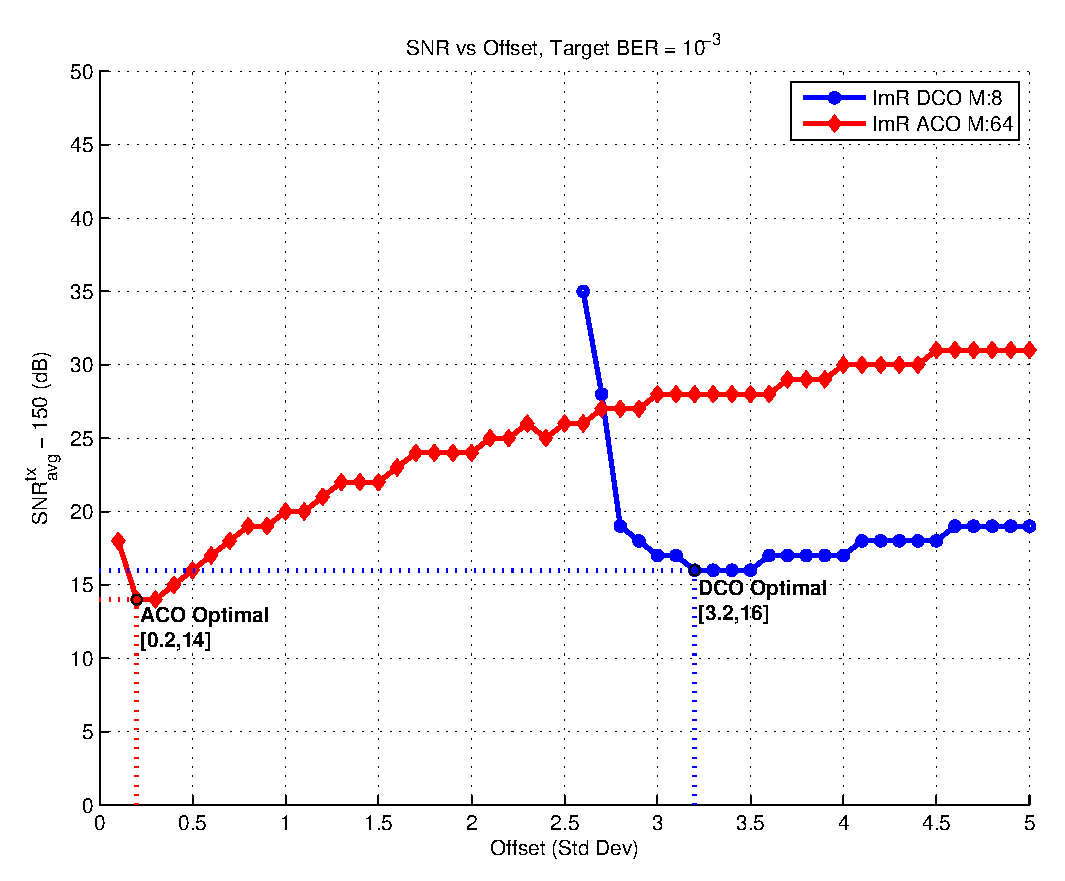
\includegraphics[trim={0in -0.1in 0in 0.0in}, clip=true, width=\textwidth]{figSNRvsOfst.eps}
\caption{SNR vs Offset for target BER $= 10^{-3}$ using an imaging receiver}
	\label{fig:SNRvsOfst}
\end{figure}

Different SIS-OFDM systems are compared at their optimal DC offsets as empirically determined from \figurename{ \ref{fig:SNRvsOfst}}. BER vs SNR curves at optimal DC offsets equal to $0.2\times$SD for ACO-OFDM with 64-QAM subcarrier modulation and $3.2\times$SD for DCO-OFDM with 8-QAM subcarrier modulation using imaging receiver and non--imaging receiver are illustrated in \figurename{ \ref{fig:BERnet}}. 
\begin{figure}[!t]
\centering
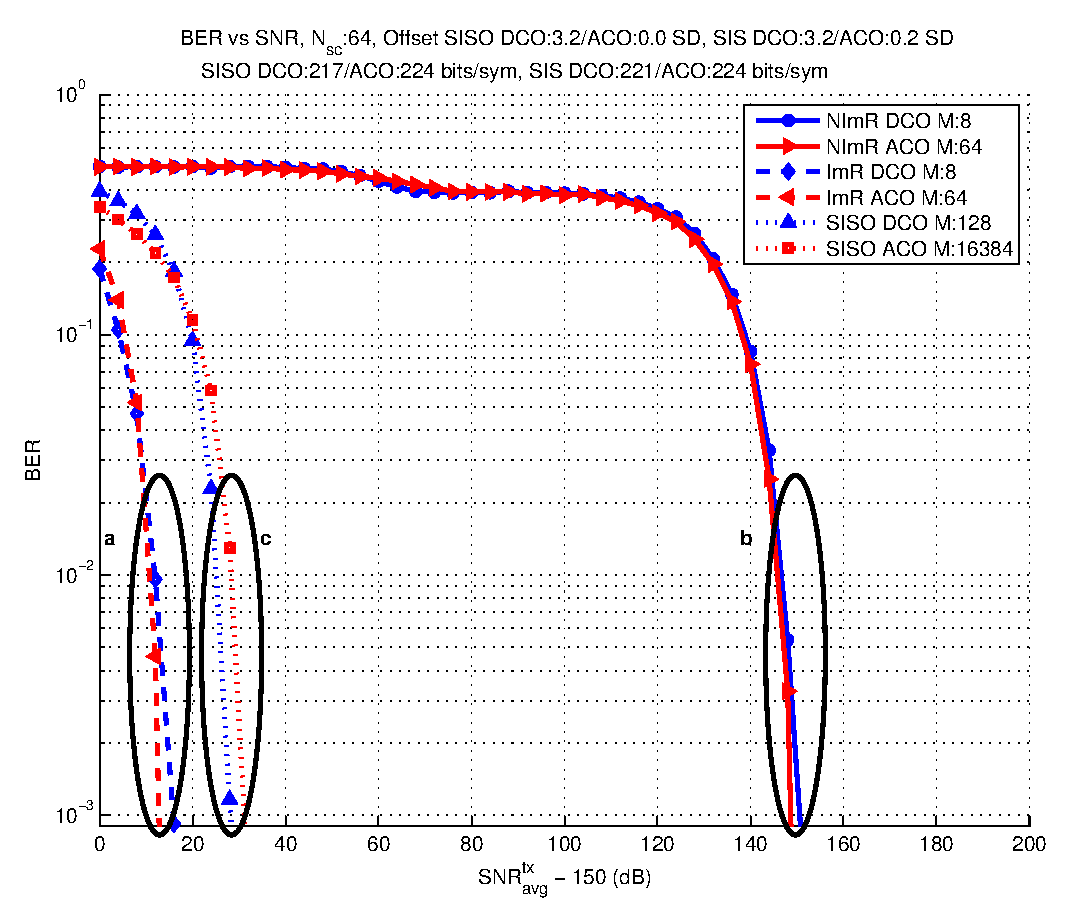
\includegraphics[trim={0.45in 0.15in 0.7in 0.00in}, clip=false, width=0.7\textwidth]{fig_35_64_all.eps}
\caption{Comparison of BER vs SNR for (a) imaging receiver, (b) non--imaging receiver and (c) SISO}
	\label{fig:BERnet}
\end{figure}
It is shown that using imaging receiver can provide significant SNR gain ($\approx$135dB) over non--imaging receiver for BER $=10^{-3}$. For the non--imaging receiver, each PD receives significant signal from each of the 4 luminaires and thus high ICI is expected. The imaging receiver provides channel decorrelation thus significantly improving the system performance. As seen from the figure, it is impractical to achieve $\approx$150dB SNR for SIS-OFDM with non--imaging receiver. The above SIS-OFDM configurations are compared with reference SISO O-OFDM systems. To achieve nearly the same bits/symbol as in the SIS-OFDM systems, DCO-OFDM with 128-QAM subcarrier modulation and ACO-OFDM with 128$^2$-QAM subcarrier modulation yielding 217 and 224 bits/symbol are required. It is impractical to achieve $\approx$30dB SNR to achieve target BER performance at comparable spectral efficiencies for SISO O-OFDM systems with higher order subcarrier modulation. The SIS-OFDM system with imaging receiver not only provides better spectral efficiency but also achieves the target BER at lower transmit powers. Additionally, the imaging receiver considered has practical dimensions and can be incorporated in portable devices.

\begin{figure}[!t]
\centering
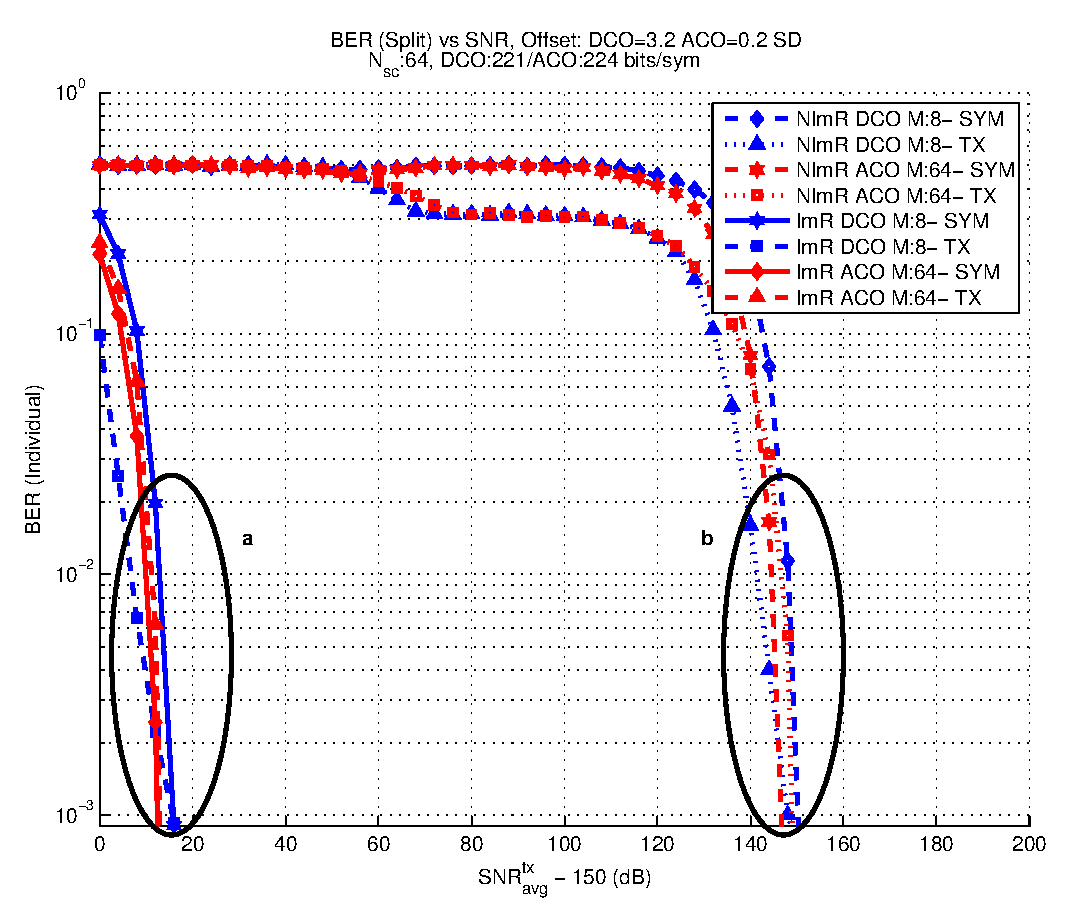
\includegraphics[trim={0.45in 0.15in 0.7in 0.00in}, clip=false, width=0.7\textwidth]{fig_35_64_all_s.eps}
\caption{Comparison of individual BER vs SNR for (a) imaging receiver and (b) non--imaging receiver}
	\label{fig:BERsplit}
\end{figure}

BER vs SNR curves for individual O-OFDM and OSM streams for the SIS-OFDM systems considered are shown in \figurename{\ref{fig:BERsplit}}. At low SNR, bit errors are dominated by errors in luminaire index detection. Errors in luminaire index leads to choosing a different signal value for decoding the O-OFDM signal, thus introducing additional errors in O-OFDM signal decoding. As the SNR increases, errors in transmitter index detection significantly decrease and errors in O-OFDM symbol decoding dominates the BER. As the SNR is further increased, errors in the O-OFDM symbol decoding decrease thus reducing the overall BER.

In conclusion, it is shown that a system implementing SIS-OFDM can achieve additional $R^{\text{s}}=N_{\text{sc}}\times $ log$^{ }_{2}(N_{\text{tx}})$ bits per symbol of spectral efficiency as compared to SISO O-OFDM systems. Results indicate that the use of an imaging receiver provides additional channel decorrelation and can help achieve up to 130 dB improvement in SNR when compared to system performance using a non--imaging receiver. At significantly lower computational complexity, the SIS-OFDM can provide an additional ($3\times N_{\text{sc}}\times k/4$) bits per symbol for ACO-OFDM and $((N_{\text{sc}}/2 -1)\times k)$ bits per symbol for DCO-OFDM over recently proposed approaches that combine OSM with O-OFDM.
